\chapter*{Annexes}
\addcontentsline{toc}{chapter}{Annexes}
\section*{Liens utiles}
\begin{itemize}
\item[]
\item \textbf{Projet GitHub} : https://github.com/open-orchestra
\item[]
\item \textbf{Site de présentation d'Open Orchestra} : open-orchestra.com
\item[]
\item \textbf{Démonstration d'Open Orchestra} : open-orchestra.com/demo
\end{itemize}
\section{Aperçus}


    \begin{figure}[H]
        \begin{center}
          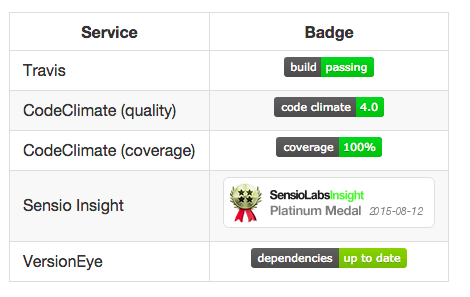
\includegraphics[scale=0.75]{images/annexe_note}
        \end{center}
        \caption{Badges de qualité d'un bundle Open Orchestra}
        \label{annexe_note}
      \end{figure}
      

     \begin{figure}[H]
          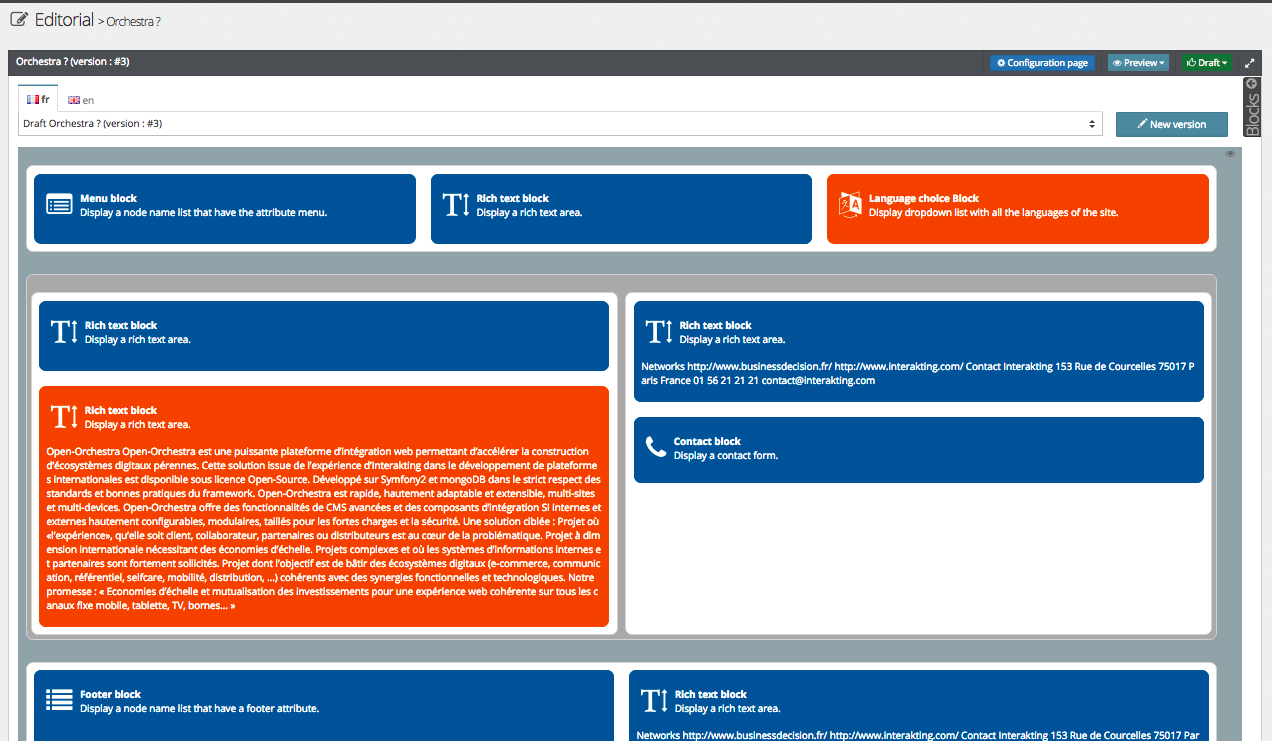
\includegraphics[scale=0.4]{images/annexe_node}
 
        \caption{Exemple de création d'un node avec des blocs}
        \label{annexe_node}
      \end{figure}
     \begin{figure}[H]
        \begin{center}
          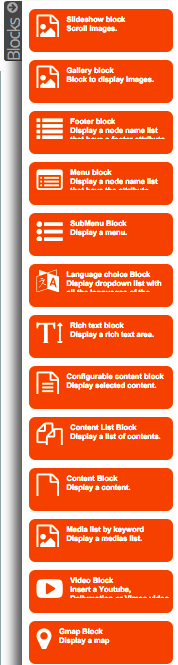
\includegraphics[scale=0.6]{images/annexe_bloc}
        \end{center}
        \caption{Liste des blocs disponible par défaut}
        \label{annexe_bloc}
      \end{figure}